\documentclass[11pt]{article}
\usepackage[utf8]{inputenc}
\usepackage{amsmath}
\usepackage{amssymb,amsfonts,latexsym,cancel}
\usepackage{graphicx}
\usepackage{epstopdf}
\usepackage{tabularx} 
\usepackage{float}
\usepackage{verbatim}
\usepackage[left=2cm, right=2cm, top=2cm, bottom=2cm]{geometry}
\setlength\parindent{0pt}
\setlength{\parskip}{2mm}

\title{MultiFEBE \\ME-ST-SR-002 [TUTORIAL] \\ \textbf{Rectangular Plate (FEM model)}}
\author{Samuel González-Jiménez and Jacob D. R. Bordón}
\date{September 2025}

\begin{document}
	\maketitle
	
	\section*{Problem description}
	In this validation case a static analysis of the Rectangular Plate problem~\cite{MacNeal1985} is performed using the Finite Element Method. As shown in Figure \ref{Rect_plate} the problem consist in a rectangular plate of a=2 in and b=2 in and a thickness of 0.0001 in. The properties of the material are a Young modulus (E) of $1.7472 \times 10^{7}  \ \text{lbf}/\text{in}^2$ and a Poisson ratio ($\nu$) of 0.3. All the boundaries of the plate are clamped and it is subjected to two different types of loads: a uniform pressure of $q=10^{-4} \  \text{lbf}/\text{in}^2$ and a central load of $P=4.0 \times 10^{-4}$ lbf. The mesh is $N \times N$ on shaded area.
	
	
	\begin{figure}[H]
		\centering
		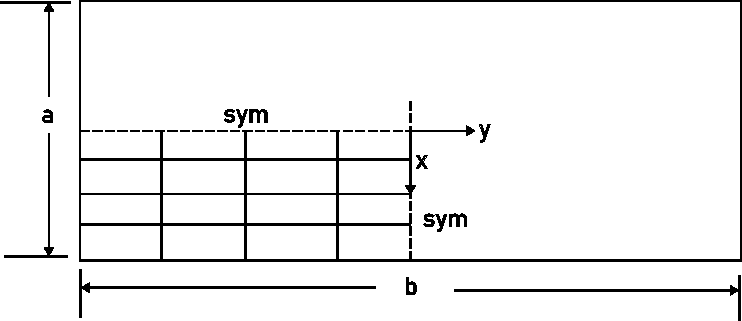
\includegraphics[scale=0.65]{Rectangular_plate_draw.pdf}
		\caption{Rectangular Plate problem}
		\label{Rect_plate}
	\end{figure}
		
	
	\section*{Input data file}
	In this section, the principal sections of the MultiFEBE input data file  will be reviewed.
	The first block to be dealt is the settings one. In this case the mesh is imported from another file named \texttt{"Rectangular\_plate.msh"} in the Gmsh MSH format version 2.2.
	
	\begin{verbatim}
	[settings]
	mesh_file_mode = 2 "Rectangular_plate.msh"
	\end{verbatim}
	
	In the section [symmetry], two planes of symmetry are defined, since only a quarter of the problem is meshed, as shown in Figure \ref{Rect_plate}. To the correct recognition of the symmetry planes, each axis of symmetry must intersect the origin of coordinates.
		
	\begin{verbatim}
	[symmetry planes]
	plane_n1: symmetry
	plane_n2: symmetry
	\end{verbatim}
		
	In the section [export], it is defined that only the nodal solutions for node 1 were displayed, where the convergence study will be performed.

	\begin{verbatim}
	[export]
	nso_nodes= 1, 1
	\end{verbatim}
		
	Since the problem is solved with Shell finite elements, in the [cross sections] section are defined the number of fe subregions related to the cross section (1), fe subregion identifier (1), type of cross section (degshell), thickness (0.0001) and reference vector for x' direction (0. 0. 1.).
	
	\begin{verbatim}
	[cross sections]
	1
	degshell 1 1 1.d-4 0. 1. 0.}
	\end{verbatim}
	
	In the [groups] section, 4 groups are defined. The group 1 and 2 selects the nodes in XZ plane at x=1 and the nodes in YZ plane at y=1 where the clamped supports conditions are applied respectively. The group 3 and 4 are composed by all the elements and nodes respectively.
	
	
	\begin{verbatim}
	[groups]
	4
	1 nodes box interior 0.99d0 1.01d0 -100.d0 100.d0 -100.d0 100.d0 1
	2 nodes box interior -100.d0 100.d0 0.99d0 1.01d0 -100.d0 100.d0 1
	3 elements all
	4 nodes all
	\end{verbatim}
	
	In the [fem node options], it is defined that all the nodes results are displayed with 6 degrees of freedom instead of 5 as established by default for shell elements.
	
	\begin{verbatim}
	[fem node options]
	group 4 n_dof 6}
	\end{verbatim}
	
	\subsection*{Uniform pressure}
	
	For the uniform pressure case the following conditions are applied:
	
	In [conditions over nodes] section, the loads are applied in their respective axes.
		\begin{verbatim}
[conditions over nodes]
group 1: 0 0
         0 0
         0 0
         0 0
         0 0
         0 0

group 2: 0 0
         0 0
         0 0
         0 0
         0 0
         0 0
	\end{verbatim}
		

	In [conditions over fe elements] all the elements are loaded with the uniform pressure.\\
	
	\texttt{[conditions over fe elements]\\
		group 3: global\\
		\hspace*{1.8cm} 0.d0 0.d0 1.d-4}
		
	\subsection*{Central load}
	
	For the central load case the following conditions are applied:
	
	In [conditions over nodes] section, the same clamped supports conditions are applied as in the previous case. Furthermore a central load in the Z-axis is applied in the central node. Note that the force is a quarter that the applied in the problem, since due to symmetry, the corresponding node has only a quarter of the stiffness of the entire problem.
	
	\begin{verbatim}
[conditions over nodes]
group 1: 0 0
         0 0
         0 0
         0 0
         0 0
         0 0
	
group 2: 0 0
         0 0
         0 0
         0 0
         0 0
         0 0
         
node 1:  0 0
         0 0
         1 1.d-4
         0 0
         0 0
         0 0
	\end{verbatim}
			
	\section*{Results and discussion}
	
	In this section the results for the convergence of an NxN study of both load cases is shown. In total 20 meshes were tested for each load case, with 2, 4, 8 and 16 elements and 5 different types of elements, i.e. MITC3i, MITC6a, MITC8* and MITC9 (see \cite{Bathe2006}). The characteristics of each type of element is shown in Table \ref{MITC_tab}.
	
	\begin{table}[H]
	\caption{Element types characteristics}
	\label{MITC_tab}
	\centering
	\begin{tabular}{|c|c|c|}
		\hline
		\textbf{Element} & \textbf{Element shape} & \textbf{Order} \\
		\hline
		MITC3i & Triangular & Linear \\
		\hline
		MITC6a & Triangular & Quadratic \\
		\hline
		MITC4 & Quadrilateral & Linear \\
		\hline
		MITC8* & Quadrilateral & Quadratic \\
		\hline
		MITC9 & Quadrilateral & Quadratic \\
		\hline
	\end{tabular}
\end{table}
	
	Figures \ref{midside_unif} and \ref{midside_centr} display the convergence of central vertical displacement of the plate for a uniform pressure load and a central point load, respectively to the reference values as a function of the number of elements. The theoretical reference values are 1.26 in for the uniform pressure case and 5.60 in for the central load case.
	
	\begin{figure}[H]
		\centering
		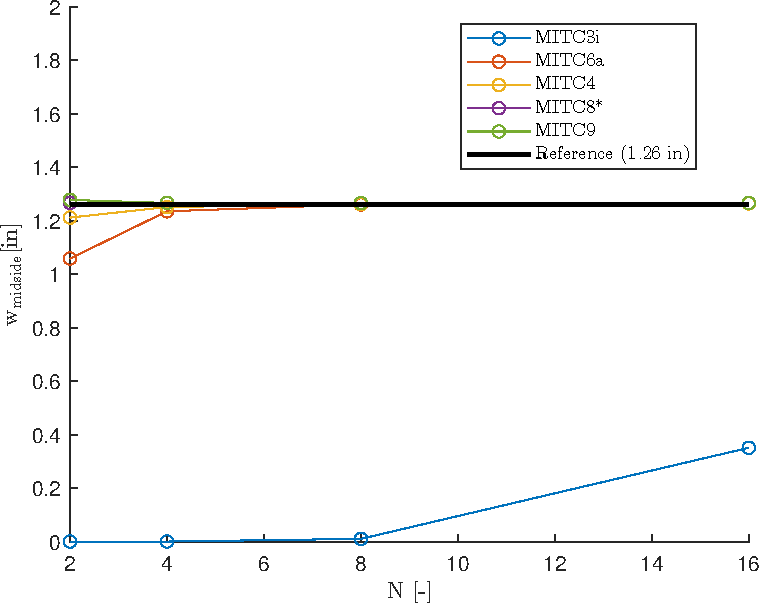
\includegraphics[scale=0.90]{w_midside_force_applicationUniform.pdf}
		\caption{Displacement at centre of plate for uniform pressure case.}
		\label{midside_unif}
	\end{figure}
	
		\begin{figure}[H]
		\centering
		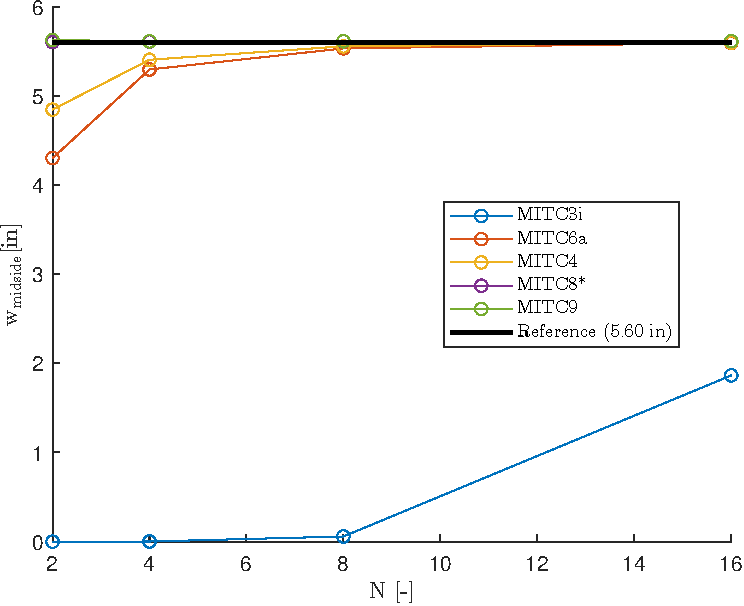
\includegraphics[scale=0.90]{w_midside_force_applicationConcentrated.pdf}
		\caption{Displacement at centre of plate for central load.}
		\label{midside_centr}
	\end{figure}
	
	In both load cases is observed that, except for case MITC3i, convergence is almost complete at 8 elements, with a faster convergence for cases MITC8* and MITC9. The MITC3i has worse convergence due to the extremely large edge length / thickness ratio (a/t = b/t = 20000).
	
	\subsection*{Deformed Shape in Gmsh}
	
To visualize the deformed shape of the meshed plate, follow these steps:
\begin{enumerate}
	\item Open the \textbf{.pos} file in Gmsh.
	\item In the \textbf{Post-processing} window, mark only the \textbf{Solid UX, UY, UZ} option.
	\item Access the menu \textbf{Tools}  $\gg$ \textbf{Options}  $\gg$ \textbf{View [0]} (corresponding to displacements).
	\item Within the view options, in the \textbf{Aspect} section, select \textbf{Displacement} under \textit{Vector display}.
	\item Adjust the \textit{Displacement factor} to \textbf{0.15}.
	\item To adjust the mesh visibility, access the menu \textbf{Tools}  $\gg$ \textbf{Options}  $\gg$ \textbf{Mesh}.
	\item In the mesh options, select only \textbf{2D element faces}.
\end{enumerate}
	By following the steps above with the correct orientation, it will be obtained a visualization similar to Figure~\ref{deformed_shape}.
	
	
	\begin{figure}[H]
		\centering
		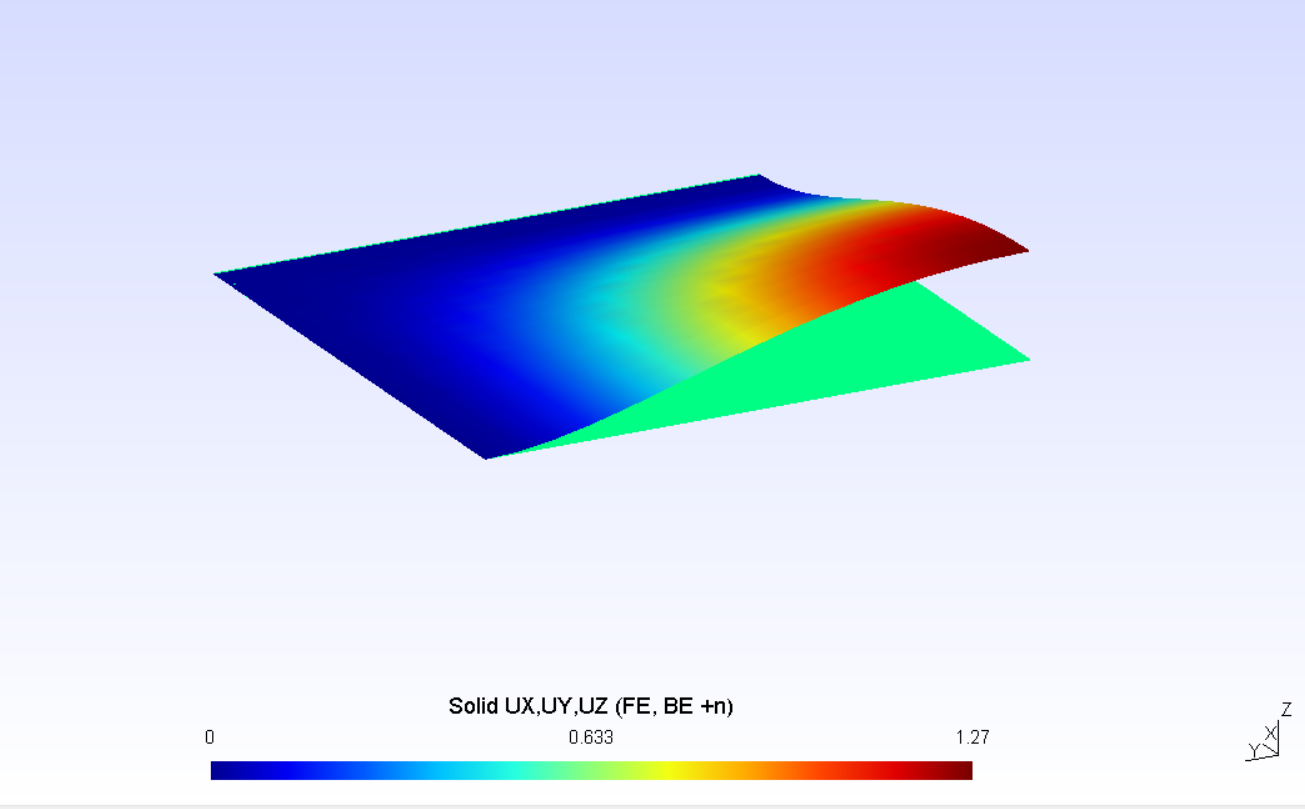
\includegraphics[scale=0.40]{Rectangular-plate deformed shape}
		\caption{Deformed shape of the quarter of plate for the MITC9 case.}
		\label{deformed_shape}
	\end{figure}
	
	
	\section*{Attachments}
	 
	 For this validation case, the convergence study execution file is attached as well as the .dat, .mesh and the .geo file. 	 
	 
	 \bibliographystyle{unsrt}
	 \bibliography{references.bib}
	 
	 \end{document}